%%%%%%%%%%%%%%%%%%%%%%%%%%%%%%%%%
% 6CCS3PRJ Final Year Individual Project Report
% luke.day@kcl.ac.uk
%%%%%%%%%%%%%%%%%%%%%%%%%%%%%%%%%
\documentclass[12pt]{informatics-report}
\usepackage{color}
\usepackage[square,sort,comma,numbers]{natbib}
\usepackage[utf8]{inputenc}
\usepackage{listings}
\usepackage{indentfirst}
\definecolor{dkgreen}{rgb}{0,0.6,0}
\definecolor{gray}{rgb}{0.5,0.5,0.5}
\definecolor{mauve}{rgb}{0.58,0,0.82}
\usepackage{float}
%\floatstyle{boxed} 
%\restylefloat{figure}
\lstset{frame=single,
  language=Java,
  aboveskip=3mm,
  belowskip=3mm,
  showstringspaces=false,
  columns=flexible,
  basicstyle={\small\ttfamily},
  numbers=none,
  numberstyle=\tiny\color{gray},
  keywordstyle=\color{blue},
  commentstyle=\color{dkgreen},
  stringstyle=\color{mauve},
  breaklines=true,
  breakatwhitespace=true,
  tabsize=3
}
 %References
%%%%%%%%%%%%%%%%%%%%%%%%%%%%%%%%%
% Front Matter - project title, name, supervisor name and date
%%%%%%%%%%%%%%%%%%%%%%%%%%%%%%%%%
\title{6CCS3PRJ\\\vspace{0.2cm}Indoor Positioning System}
\author{Sari Nusier}
\studentID{1317015}
\supervisor{Dr. Andrew Coles}

\date{\today}

\abstractFile{FrontMatter/abstract.tex}
\ackFile{FrontMatter/acknowledgements.tex} %Remove line if you do not want acknowledgements

\begin{document}
\createFrontMatter
\onehalfspacing
\tableofcontents
\doublespacing

%%%%%%%%%%%%%%%%%%%%%%%%%%%%%%%%%
% Report Content
%%%%%%%%%%%%%%%%%%%%%%%%%%%%%%%%%
% You can write each chapter directly here or in a separate .tex file and use the include command.

\chapter{Introduction}
This is one of the most important components of the report. It should begin with a clear statement of what the project is about so that the nature and scope of the project can be understood by a lay reader. It should summarise everything that you set out to achieve, provide a clear summary of the project's background and relevance to other work, and give pointers to the remaining sections of the report, which will contain the bulk of the technical material.

\section{Motivation}
Visiting multiple museums has led me to notice that, even though there are maps and guides available, there is no simple way of going on a self guided tour. Another issue was that most of the details provided about the exhibits are delivered through audio guides, with no options available for hearing impaired people. These issues can be solved by developing a digital guide.

In order to implement such a system, the visitor must be aware of its location at all times. This has led me to discover the existence of the concept of context aware systems, and the problem that indoor positioning poses to the implementation of such systems. After some research, I have come to the conclusion that, even though there are many studies that try to solve the problem of indoor positioning, no universal solution can be found, and the number of available systems is limited. In a museum guide application, as in other similar applications, accuracy is not a necessity, even less so if it affects precision. Therefore my decision was to try and develop a system that identifies only the room in which a person is located, instead of the actual coordinates in space. This will hopefully increase the precision of the system, giving the correct results more often than if the system were to predict a more accurate location.

\section{Project Scope}
Due to the lack of GPS availability in indoor environments, a different approach to positioning must be taken. The project examines the performance and feasibility of applying Machine Learning classification in the context of indoor positioning. The classifiers are created using the widely available Wi-Fi infrastructure. Received Signal Strength measurements of all visible Access Points will be taken inside each room, creating a “fingerprint” which can be later used to determine in which room a measurement was taken. Even though the project uses Wi-Fi signal strength as the means to creating “fingerprints”, the positioning system is developed to work independent of the measuring system, other signal types or distance measurements can be used.
The project will also implement a solution to the orienteering problem, being able to suggest routes based on visitor preference and time constraints.
The system developed is composed of multiple subsystems, from user interface to the backend implementing the positioning and orienteering algorithms. The subsystems will be as independent as possible, to reduce the impact on the system as a whole when changes are made in the subsystems.

\section{Objectives}
The resulting system must be easy to use and offer a starting point for future work. Basic interfacing with the system will be made through two Android applications. The application should store the data inputted by the users in a simple to parse format. The Backend server and the positioning and orienteering systems must be independent and run as separate instances on a machine, allowing for more flexibility.
Below are the main objectives summarised:
\begin{enumerate}
\item Create two android apps that will allow for users to interact with the system. The Administration app should be easy to use and allow hosts to create and manage the data. The Visitor app should display user’s location and suggest a route to follow for their visit.
\item Create a server that runs the management of the positioning and orienteering system.
\item Create a Restful API and a Database to manage and store the content provided by the other subsystems. It should provide a way to store data and forward requests from the apps to the positioning and orienteering system.
\end{enumerate}

\section{Report Structure}
The report's body is split into 9 chapters, including the Introduction.
Chapter 2, Background, will discuss current approaches to positioning for both outdoors and indoors, focusing more on the indoors part, as it is more relevant. It will also discuss the tools used for orienteering and give a little bit of background on Machine Learning and classifiers. 

Chapter 3 will define the Requirements of the system and will then show what approaches will be taken in order to meet those requirements.

Chapter 4 will look into the design of the entire system and the interaction between its components. Moreover, it will look in more detail at the design of each subsystem, providing an aid to the implementation phase.

Chapter 6 will discuss the Software development approach used during the implementation of the software. It will then list the steps taken to develop the resulting system, provide a detailed description of the implementation of each subsystem and briefly discuss some of the problems encountered during the process.

Chapter 7 will evaluate the resulting software by comparing it with the requirements and design defined in the previous chapters. In addition, it will evaluate the precision of the Machine Learning approach to positioning by showing some statistical data collected during testing. Finally, it will look at how the software was tested to avoid possible bugs and to ensure a feasible end result.
 




\chapter{Background}

\section{Global Positioning System}
"GPS answers the questions 'What time, what position, and what velocity is it?' quickly, accurately, and inexpensively anywhere on the globe at any time" (Hofmann-Wellenhof, Lichtenegger and Collins, 1997).  

In order to locate aircrafts and ships, the U.S. military developed a system called TRANSIT, the predecessor of the modern positioning system. It used six satellites at an altitude of 1,100 km, passing over one point on earth roughly every 90 minutes. The system worked by using the Doppler effect, the change of a wave's frequency for an observer relative to movement, to compute its location. This meant that users had to wait between "fixes" quite a long period, making the system unusable for real-time positioning, but enough for military applications (Hofmann-Wellenhof, Lichtenegger and Collins, 1997). 

GPS solved this problem by ensuring that at least four satellites were always electronically visible. This allows for a receiver to compute its location using trilateration. The increase in accuracy and the ability to find one’s location in real-time, made the GPS suitable for civilian applications. 

Due to a higher complexity of indoor environments and the lack of line-of-sight transmissions between the receiver and the satellites, GPS is not suitable for indoor applications (Gu, Lo and Niemegeers, 2009).

\section{Indoor Positioning System}
”In the last years a great deal of research has been conducted on developing methods and technologies for automatic location-sensing of people or devices” [3]. Like the GPS, an IPS is a system that continuously and in real-time can determine the position of something or someone in a physical space [5]. Unlike GPS, IPS must be available for indoor environments [2]. 

\subsection{General}
Hightower and Borriello [4] define three Location Sensing Techniques: Triangulation, Scene Analysis and Proximity. 
Triangulation can be made through lateration or angulation. For the lateration approach, distance from the device to three or four points (non-collinear/non-coplanar) must be measured. Using a direct form of measurement is the most accurate and straightforward solution, but very hard to implement in an automated system. Another approach is the use of Time-of-Flight, the time taken to reach the reference point, knowing the velocity. When using radio waves to calculate distance, one problem is regarding time synchronisation. Because indoor environments are usually small, the smallest time discrepancy can greatly affect accuracy. Another problem that might arise is when the same pulse arrives at different times, due to reflections. Attenuation can also be used to calculate distance. That is, the signal strength decrease over the travelled distance. “In environments with many obstructions such as an indoor office space, measuring distance using attenuation is usually less accurate than time-of-flight” [4].
Proximity location sensing determines if a device is near a known point. This can be detected through physical contact or using the limited ranges of Radio transceivers, such as Wi-Fi access points. Another way of determining proximity can be through user interaction. For example in a museum, if each exhibition has a QR code or an NFC card for the user to interact with, a scan of the two can imply that the user is viewing the exhibit and is near it.

Proximity location sensing determines if a device is near a known point. This can be detected through physical contact or using the limited ranges of Radio transceivers, such as Wi-Fi access points. Another way of determining proximity can be through user interaction. For example in a museum, if each exhibition has a QR code or an NFC card for the user to interact with, a scan of the two can imply that the user is viewing the exhibit and is near it.
\subsection{Fingerprinting}
Kaemarungsi and Krishnamurthy [6] review the use of WLAN Location Fingerprinting as a way of locating a device in physical space. Small, A. Smailagic, and D. P. Siewiorek [7] found that the distribution of RSS in dB from Wi-Fi access points follows a Gaussian Distribution. Kaemarungsi and Krishnamurthy [6] argue that this might be due to the lack of user presence when the measurements were taken. They have found that, when a user is present, the distribution was non-Gaussian and asymmetric. They conclude that it is a better approach to record the distribution of RSS rather than calculate and use the mean value. 
Battiti, M. Brunato [8] use Statistical Learning to determine the location of devices. The first use Bayesian Approach, WKNN and Support Vector machines to solve the location positioning as a regression problem. Another approach taken, close to the approach used in this project, was to consider positioning as a classification problem, labeling each room in the building and using a learning set for each room. Out of 257 measurements, they found the following results:
\begin{itemize}
\item SVM: classifier: 8 errors, regression: 20 errors.
\item Multilayer perceptron: classifier: 34 errors, regression: 31 errors.
\item WKNN: regression: 15 errors
\item Bayesian regression: 33 errors.
\end{itemize}
These results will be used to compare with the end results of this project.

\section{Machine Learning}

"The field of pattern recognition is concerned with the automatic discovery of regularities in data through the use of computer algorithms and with the use of these regularities to take actions such as classifying the data into different categories". (Bishop, 2006)
One part of machine learning is concerned with supervised learning, in which the training data is a set of input vectors, given along with their corresponding target vectors. When the goal is to associate each input vector to one of a finite set of categories, it is called a classification problem. Understand of the mathematics behind the classifiers used in the project is not needed for implementation, as the classifiers are implemented using the Weka Library, but it might help choosing which classifier to be used when predicting location based on RSS. Even though this project will use a statistical approach to picking the best classifiers, limited mathematical definitions of the some classifiers will be included below. For more details, a great source is Bishop [10].

\subsection{Naive Bayes classifiers}
This is one of the most popular approach to classifiers. Murphy [9] states that,even though usually false, the assumption made by Naive Bayes is that all the features are conditionally independent given the class label:
$$ p(x|y = c) = \prod\limits_{i=1}^D p(x_i|y = c) $$

As we have seen in the previous section (2.2.2), the data containing the RSS is usually Gaussian distributed, especially when a user is not present as the measurements are not taken. In this case, we get:
$$ p(x|y = c,\theta_c) = \prod\limits_{i=1}^D \mathcal{N}(x_i|\mu_{ic} = \sigma_{ic}) $$ and must estimate $C \times D$ separate Gaussian parameters, $\mu_{ic}$, $\sigma_{ic}$, where $C$ is the set of class labels and $D$ is the set of features, as real numbers [9].

\subsection{Bayesian Networks}
When a large number of variables are used, such as in our case, many Access Points, it is not efficient to represent the dependencies between each variable. To solve this, a graph can be built to represent those dependencies, by describing complex joint distributions using local distributions. In other words, we can see how variables interact locally, and chain these interactions to see the global interaction.
Consider an arbitrary joint distribution $p(a,b,c)$ over three variables $a$, $b$, and $c$.
By applying the product rule of probability, $p(X,Y) = p(Y|X)p(X)$ the joint distribution will become $$p(a,b,c) = p(c|a,b)p(a,b)$$
A second application of the product rule, this time to the second term on the righthand gives $$p(a,b,c) = p(c|a, b)p(b|a)p(a)$$
We now represent the right side of the equation as a graph by introducing a node for each variable and associate each node with the corresponding conditional distribution. That is, $c$ is dependent on $a$ and $b$, $b$ is dependant on $a$ and $a$ is independent. A general example can be considered for the joint distribution over $K$ variables given by $p(x_1,x_2,...,x_K)$. As seen before, the joint distribution can be written as: $p(x_1,...,x_K) = p(x_K|x_1,...,x_{K-1})...p(x_2|x_1)p(x_1)$



\chapter{Requirements and Specifiations}
\noindent The HOST represents the management of the building implementing the positioning system.\\ 
The VISITOR is any user of the positioning app, regardless of the building they are visiting.
Both users will require Wi-Fi enabled Android Devices and a stable internet connection.

\section{Requirements}
The requirements are split in four categories. The first two are concerned with user requirements from both HOST and VISITOR perspective. The positioning system is the software that handles data analysis and machine learning to provide the position of the VISITOR. In addition, the positioning server is used to generate visitor routes and approximate visit times.

\subsection{Host requirements}
	\begin{itemize}
		\item H1 - Host must be able to create, edit, remove or view buildings.
		\item H2 - Host must be able to create, edit, remove or view rooms from a specified building.
		\item H3 - Host must be able to measure WiFi APs signal strength for a specified room.
		\item H4 - Host must be able to train, update or reset the positioning system with new measurements.
	\end{itemize}

\subsection{Visitor requirements}
	\begin{itemize}
		\item V1 - Manually select a building to visit.
		\item V2 - Receive a suggestion regarding the building they are in.
		\item V3 - Choose the rooms/exhibits they would like to visit inside a building.
		\item V4 - Receive an estimated time of visit based on selected rooms/exhibits.
		\item V5 - Rate the importance of visiting a specific room/exhibit.
		\item V6 - Receive a suggested visit path based on selected rooms/exhibits.
		\item V7 - See its current location within the building.
		\item V8 - See a visit path based on its current location and the selected rooms/exhibits.
		\item V9 - Display the current exhibit being viewed, based on proximity sensing.
	\end{itemize}

\subsection{Positioning requirements}
	\begin{itemize}
		\item PS1 - Receive a learning set containing AP signal strength measurements and the 	location they were taken in.
		\item PS2 - Create classifiers from learning set.
		\item PS3 - Receive unclassified data containing AP signal strength measurements.
		\item PS4 - Classify received data using one or more previously built classifiers.
		\item PS5 - Return classified data in a format that can be easily parsed by the user.
		\item PS6 - Receive visitor requirements as a list of selected rooms, how much the visitor wants to visit each room and a deadline.
		\item PS7 - Generate and return a route based on the requirements received from the user.
	\end{itemize}

\subsection{Backend requirements}
	\begin{itemize}
		\item B1 - Database should store buildings and the rooms within each building. 
		\item B2. Database should store the learning set for each building and other important data.
		\item B3. Server should maintain a RESTful API to interface with the database and positioning 			system.
	\end{itemize}


\section{Specifications}
The specifications show what should be implemented in order to meet the requirements of the software.

\subsection{Host}
For requirements H1 to H4 an Android application will be developed for the administration of the buildings created by a HOST:
	\begin{itemize}
		\item Activity to view all the buildings available. (H1)
		\item Activity to add a new building. (H1)
		\item Activity for the management of a specific building. (H - 1, 2, 4)
		\item Activity for the management of a specific room. (H - 2, 3)
		\item Make HTTP requests and receive data from the Backend.
	\end{itemize}

\subsection{Visitor}
For requirements V1 to V9 an android application will be developed as follows:
	\begin{itemize}
		\item Activity to view all the buildings available. (V1)
		\item Move the current building, if detected, to the top of the list. (V2)
		\item An activity containing a list of exhibits/rooms inside a building. (V3)
		\item Compute the sum of the estimated visit time of all the selected rooms. (V4)
		\item Implement a seekbar for each selected exhibit. (V5)
		\item Display a generated route as a text or as a path on the map. (V6)
		\item Current location should be displayed as a text or on the map. (V7)
		\item Update the suggested path based on current location. (V8)
		\item Bluetooth beacons associated to exhibits can be used to detect proximity. (V9)
	\end{itemize}

\subsection{Positioning system}
For requirements PS1 to PS5 a Java application will be developed as follows:
	\begin{itemize}
		\item Accept TCP connections to send and receive JSON data. (PS - 1, 5)
		\item Implement machine learning and JSON parsing libraries. (PS - 1, 2, 3, 4, 5)
		\item Implement planning and JSON parsing for the planner used. (PS - 6, 7)
		\item Machine Learning algorithm should take less than 10 seconds to build a model and less than 1 second to classify input data.
		\item The classifier should be able to predict the correct room more than 80\% of the time.
		\item Planner should take less than 2 seconds to generate a route.
	\end{itemize}

\subsection{Backend}
The backend should implement a database and an HTTP server to:
	\begin{itemize}
		\item Accept HTTP requests for the REST API
		\item Store data in JSON format.
	\end{itemize}

\subsection{Limitations}
When developing the system, security was not a main consideration. The system does not implement any form of authentication or access control. It does not distinguish between multiple users, all data being commonly accessible and anonymous. 
The data is available only through the REST API and any request which is not formatted correctly will be ignored. Arbitrary code execution and any type of code injections have been considered and security measures implemented.
The design of the backend is made to be extendable and any additional security measures can be easily implemented.
The look of the user interface was not a priority, therefore the design is simple, but usable. Outputs are usually plain text and visual cues are rarely given. 
The visual indoor maps and all the visual cues (location pin, walk path, etc.) are implemented using the Google Maps API, therefore available only for the buildings that have implemented Google Indoor Maps.
\chapter{Design}
\section{Architectural design}
In this section we will define the architecture of the entire system, showing the dependencies between its components. See Figure 4.1.

\begin{figure}
\noindent\makebox[\textwidth]{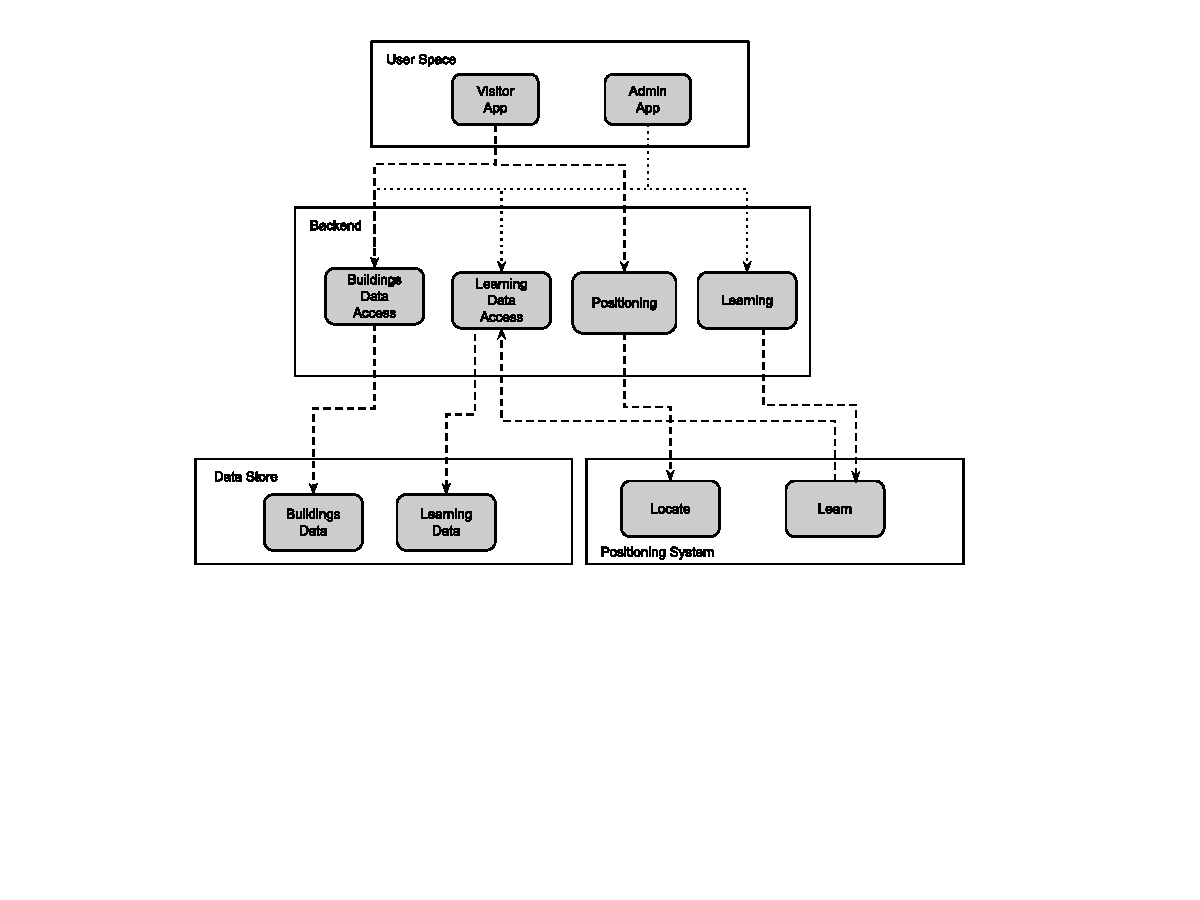
\includegraphics[clip, trim=0cm 3cm 0cm 0.7cm, width=\paperwidth]{DIAGRAMS/SystemArch.pdf}}
\caption{System Architecture}
\end{figure}
The architecture of the system is comprised of three subsystems. The top subsystem is concerned with interfacing the end users (HOST and VISITOR) to the lower subsystems. The middle subsystem offers an API to the bottom subsystems. The bottom subsystems manage and provide the information required for the entire system to run. To continue, we will review each subsystem in more detail, from top to bottom.
\clearpage
\subsection{User Space}
\noindent This layer is comprised of two Android Application, one for each type of user. The following are common features for both applications:
\begin{enumerate}
\item Implement serializable classes for the models defined in the database
\item Request and receive data from the backend in JSON format.
\item Post data to the Backend in JSON format.
\item Parse JSON data to create Java Objects
\item Convert Java Objects into JSON.
\item Activity to display all the buildings available in a ListView
\item Buildings ListView must be clickable and, on click should launch another activity for the specific building.
\item Clicking on a room should launch an activity for the selected room.
\item Implement Wi-Fi capabilities in order to measure signal strength of all visible APs.
\end{enumerate}
These common features will be implemented in packages that can be shared across the two apps.

\noindent \textbf{Administration application (HOST)}

Due to the difference in requirements a separate android application must be developed for the HOST. In addition to the common features, the application will also implement the following:
\begin{enumerate}
\item A button to add a new building In addition to the list of available buildings.
\item An add building activity containing a form and a submit button for creating a new building
\item Selecting a building from the list opens an activity containing fields that can be used to edit the building’s information.
\item A clickable ListView with all rooms in a building as part of the activity mentioned above.
\item A "learn" button to update the Positioning system with new data.
\item Clicking on an item in the Rooms ListView will open an activity that will allow the apps to measure the signal strength of all APs, associating them with the selected room, posting to the database.
\item A button in the Building activity to add new rooms.
\item The add room button will open an activity containing a form and a submit button for creating a new room.
\end{enumerate}

\noindent \textbf{Visitor application}

In addition to the common features, the visitor application will also implement the following:
\begin{enumerate}
\item A clickable ListView with all the buildings available.
\item Selecting a Building will open an activity containing a list of all rooms as selectable items. Selecting an item will update the Estimated Time value displayed somewhere below.
\item A button to start the visit will open another activity that either displays the Google Indoor Map if available, or a textview.
\item The Visit Activity displays the current location of the visitor as a pin on the Map or as text.
\item The Visit Activity displays a recommended path for the visit on the Map or as text.
\item The Visit Activity detects and displays the current exhibit beind viewed, using proximity sensing.
\end{enumerate}

\subsection{Backend}
For the simplicity of the software, and for a more efficient integration of all subsystems, the backend is ran using a NodeJS server, implementing a RESTful API.
The API handles HTTP methods to "http://serveraddress/res/", where res is the resource targeted. In addition /res/id can be used, where available, to apply method to a resource that has the specified id.
The resources available and the results of each method are as follows:
\begin{itemize}
\item For resource "buildings/":
	\begin{itemize}
	\item GET: Returns a list of all buildings stored in the database
	\item POST: Adds a new building to the database
	\end{itemize}
\item For resource "buildings/id/":
	\begin{itemize}
	\item GET: Returns the building with the specified id
	\item PUT: Updates the building with the specified id
	\item DELETE: Deletes the building with the specified id
	\end{itemize}
\item For resource "rooms/id/":
	\begin{itemize}
	\item GET: Returns the rooms that belong to the building with the specified id
	\item POST: Adds a new room to the building with the specified id
	\item DELETE: Deletes the room with the specified id
	\end{itemize}
\item For resource "measurements/":
	\begin{itemize}
	\item GET: Returns all measurements taken on the system
	\item DELETE: Deletes all measurements taken on the system
	\end{itemize}
\item For resource "measurements/id":
	\begin{itemize}
	\item GET: Returns measurements taken for the room with the specified id
	\item POST: Adds a new measurement associated to the room with the specified id
	\end{itemize}
\item For resource "learn/id":
	\begin{itemize}
	\item GET: Updates the positioning system for the building with the specified id
	\end{itemize}
\item For resource "locate/id":
	\begin{itemize}
	\item POST: Returns the predicted location in the building with the specified id
	\end{itemize}
\item For resource "route/id":
	\begin{itemize}
	\item POST: Returns the generated route, based on the requirements sent, through the building with the specified id
	\end{itemize}
\item For resource "exhibit/id":
	\item GET: Returns all exhibits in the room with the specified id as a pair of Bluetooth beacon address and Name.
	\item POST: Creates a new exhibit with the given name and address.
\end{itemize}

\subsection{Positioning System}
This is the most important part of the project. It is the software which implements the machine learning and data processing algorithms in order to create the classifiers needed for positioning.
This subsystem is built out of a X modules, each one with its own task. It is implemented using the Weka Machine Learning libraries ~\cite{Weka}. The software implements the following features:
\begin{enumerate}
\item Opens TCP connections in order to receive requests and data.
\item A JSON Object is received containing the request type and the data to be used.
\item For a request of type "learn" the software parses the data received and creates a classifier using it.
\item In order for this to happen, the software will require to convert the data into and ARFF file format.
\item A list of all the rooms is extracted and saved as a local file in JSON format. The file is named using the "building\_id"+"\_buildings.json"
\item A list of all the Reference Points (RPs) is extracted and saved as a local file in JSON format. The file is named using the building\_id + \_RPs.json
\item Using the learning set ARFF file, a classifier is initialised and added to an array for future use.
\item For a request of Type "classify", the system checks whether a classifier has been built for the building id given in the request.
\item If a classifier has been previously built but it has not been initialised in the current run of the system, the server will initialise a classifier using the data saved from the previous learn command called for the building.
\item If a classifier has never been built, the system will return an error.
\item Once the classifier is initialised, it will be used to classify the data received in the request, and will return the room as a result.
\item The system implements multiple algorithms therefore a format must be implemented to return multiple results given by different algorithms. The data is returned as follows: [algorithm\_name]:[predicted\_room\_id],[algorithm\_name]:[predicted\_room\_id], etc. In other words, the algorithm name and the room predicted by it are separated by ":" and the algorithms are separated using ",".
\item For a request of Type "route", the system parses the requirements in JSON and creates a problem file in PDDL. 
\item The problem file is then used with the predefined domain file and the OPTIC planner to generate a suggested route.
\item The data returned by the planner must also be parsed, the resulting data to be sent following the pattern:
 "view:room1;walk:room1,room2;view:room2" etc.
\end{enumerate}

\noindent When designing the system, multiple methods for finding the location of the device were considered.

\noindent \textit{\textbf{Trilateration}}

Firstly, dimensions of the building and its rooms, and the coordinates of each RP must be known. An RSS measurement is then taken for each visible RP: one next to the RP and one at the furthest corner from the RP, in the same room. To increase precision, more measurements at each of the two points can be taken and the results averaged. \\ 
We define: \\
$MRP_0$ - Average signal strength taken at the RP coordinates. \\
$MRP$ - Average signal strength taken at the furthest corner from the RP, in the same room. \\
$DRP$ - Distance (in meters) from the RP's location to where $MRP$ was taken.\\
In perfect conditions the Distance as a function of Signal Strength increases linearly. Therefore, to convert Signal Strength to Distance is a regression problem.\\
Using the equation of the line $$y = mx + n$$ we must find the gradient $m$ and the y-intercept $n$.\\
We compute $$m = \frac{DRP}{MRP - MRP_0}$$
and $$n  = DRP - m * MRP$$
$m$ and $n$ values are then saved for each RP and the distance will be calculated as $$Distance  = M * RSS + N$$
\\
To find the location of the device based on the distance measured we must find the intersection of $n$ circles (where $n$ is the number of RPs taken into account and must be greater than 3 if the coordinates must be found in 2 dimensional space, or 4 if in a 3 dimensional space).  To determine the intersection points for 3 RPs we will use the algorithm defined by Paul Bourke [8]:\\
First calculate the distance d between the center of the circles $d = |P_1 - P_0|$\\
If $d > r_0 + r_1$ or $d < |r_0 - r_1|$ then there are no solutions. If $d = 0$ and $r_0 = r_1$ then are an infinite number of solutions.\\
Considering the two triangles $P_0P_2P_3$ and $P_1P_2P_3$ we can write $$a^2 + h^2 = r_0^2$$ $$b^2 + h^2 = r_1^2$$

\noindent Using $d = a + b$ we can solve for $a$,
$$a = \frac{r_0^2 - r_1^2 +d^2}{2d}$$
It can be readily shown that this reduces to $r_0$ when the two circles touch at one point.
Solve for $h$ by substituting a into the first equation, $$h^2 = r_0^2 - a^2$$
So $$P_2 = P_0 + \frac{P_1 - P_0}{d}$$
And finally, $P_3 = (x_3, y_3)$ in terms of $P_0 = (x_0, y_0),  P_1 = (x_1, y_1) and P_2 = (x_2, y_2)$ is $$x_3 =\frac{x_2 + -h(y_1 - y_0)}{d}$$ $$y_3 =\frac{y_2 - +h(x_1 - x_0)}{d}$$
The problem with this approach is that it assumes that the distance measurements are precise. In our case, where the readings are not precise, errors can occur, such as one or more circle not intersecting in one exact point or, intersecting at all.
This can be solved by finding the closest point to all circles, such that the sum of all distances from a point to the circle be the minimum.\\
\\
\textit{\textbf{Probability based approach}}

Because the specification of the software favours precision over accuracy, it is therefore a better approach to try and guess the room in which the device is found, instead of the actual coordinates. Therefore, an approach is to calculate the probability of a device to be in a room, based on statistic data.\\
Each room must store a list of average readings for all the reference points visible from that room. 
We define:\\
\begin{itemize}
\item $AVG(RP_x, R_y)$ as the average signal strength value for $RP_x$ taken in room $R_y$.
\item $N(R_y)$ as the number of RPs that can be measured from room $R_y$.
\item $mRP_x$ as a signal strength measurement for $RP_x$.
\end{itemize} 

A reading is given as a list of $mRP$, that is, the readings taken at a moment in time. The goal is to use this list and calculate the probability that the readings were taken in a specific room.\\
For each room $R_i$, we calculate $S$ for each measurement $mRP_j$, if $AVG(RP_j, R_i)$ exists and is different than 0, as follows:
$$S(RP_j, R_i) = | 1 - \frac{mRP_j}{AVG(RPj, Ri)}|+1$$
Giving us a score from 1 to infinity.\\
We then calculate 
$$\frac{\displaystyle\sum_{i=1}^{M} \frac{1}{S(RP_i, R_x)}}{N(R_x)}$$
where $M$ is the number of measurements in the set.
The result is the probability for the measurements to have been taken in room $R_x$.
We can then compare the probability for all rooms and choose the one which is most likely.\\
\\
\textit{\textbf{Machine Learning approach}}

Machine Learning algorithms can be applied to this application in order to predict the room in which a device is located. We first define a learning set of all measurements taken and the rooms that the measurements were taken in.\\
There are five classifiers considered:
Naive Bayes, Bayes Networks, KStar, Decorate and NB Trees. The classifiers are implemented using the Weka Machine Learning Library ~\cite{Weka}. The result of each classifier is returned to the backend, therefore, the decision of which predicted value to be used is moved higher up in the system.
Due to a higher level of precision, the Machine Learning approach will have the priority in implementation.

\subsection{Data Store}
The Data Store contains two types of data, Building related and Learning related. 
Building data is all data concerning the operation and visualisation of the buildings and the rooms contained. Learning data is the data used by the Positioning System.
Initially, this layer was designed using an MySQL, but due to compatibility and performance issues with Android and longer development time, it has been changed to MongoDB.
\\
The following data models were defined to be used with the database:
\\
RECTANGLE:	
\begin{itemize}
	\item 4 coordinates (X,Y), one for each angle: Left-top (LT), Right-top (RT), Left-bottom(LB), Right-bottom (RB)
\end{itemize}

BUILDING:
\begin{itemize}
	\item Name: The name of the building as a string.
	\item Rectangle: The rectangle model that defines the building.
	\item Width and Height(length)
\end{itemize}


ROOM: 
\begin{itemize}
	\item Name: The name of the room as a string.
	\item Rectangle: The rectangle model that defines the room.
	\item Width and Height(length)
	\item Floor: The floor number in which this room is located.
	\item Estimated Time of Visit
	\item Building ID: to associate each room to a building
\end{itemize}

Reference Point (RP): This is a point in space for which distance measurements are taken.
\begin{itemize}
	\item RPID: A unique identifier
	\item Building ID: To associate each RP to a building.
	\item Coordinates (X, Y)
\end{itemize}

RP Measurement: Distance to an RP as measured in a specific room.
\begin{itemize}
	\item RP - Value Pair: Contains the RPID and the value of the measurement
	\item Room ID: The ID of the room in which the measurement was taken
\end{itemize}

\section{Data Flow and Subsystem Interaction}
Because of the vast amount of data that must be transferred between the subsystems, it is important to visualise and understand what data must be inputted in each subsystem, what data is outputted by each subsystem and how this data moves around in the entire system.
\begin{figure}
\noindent\makebox[\textwidth]{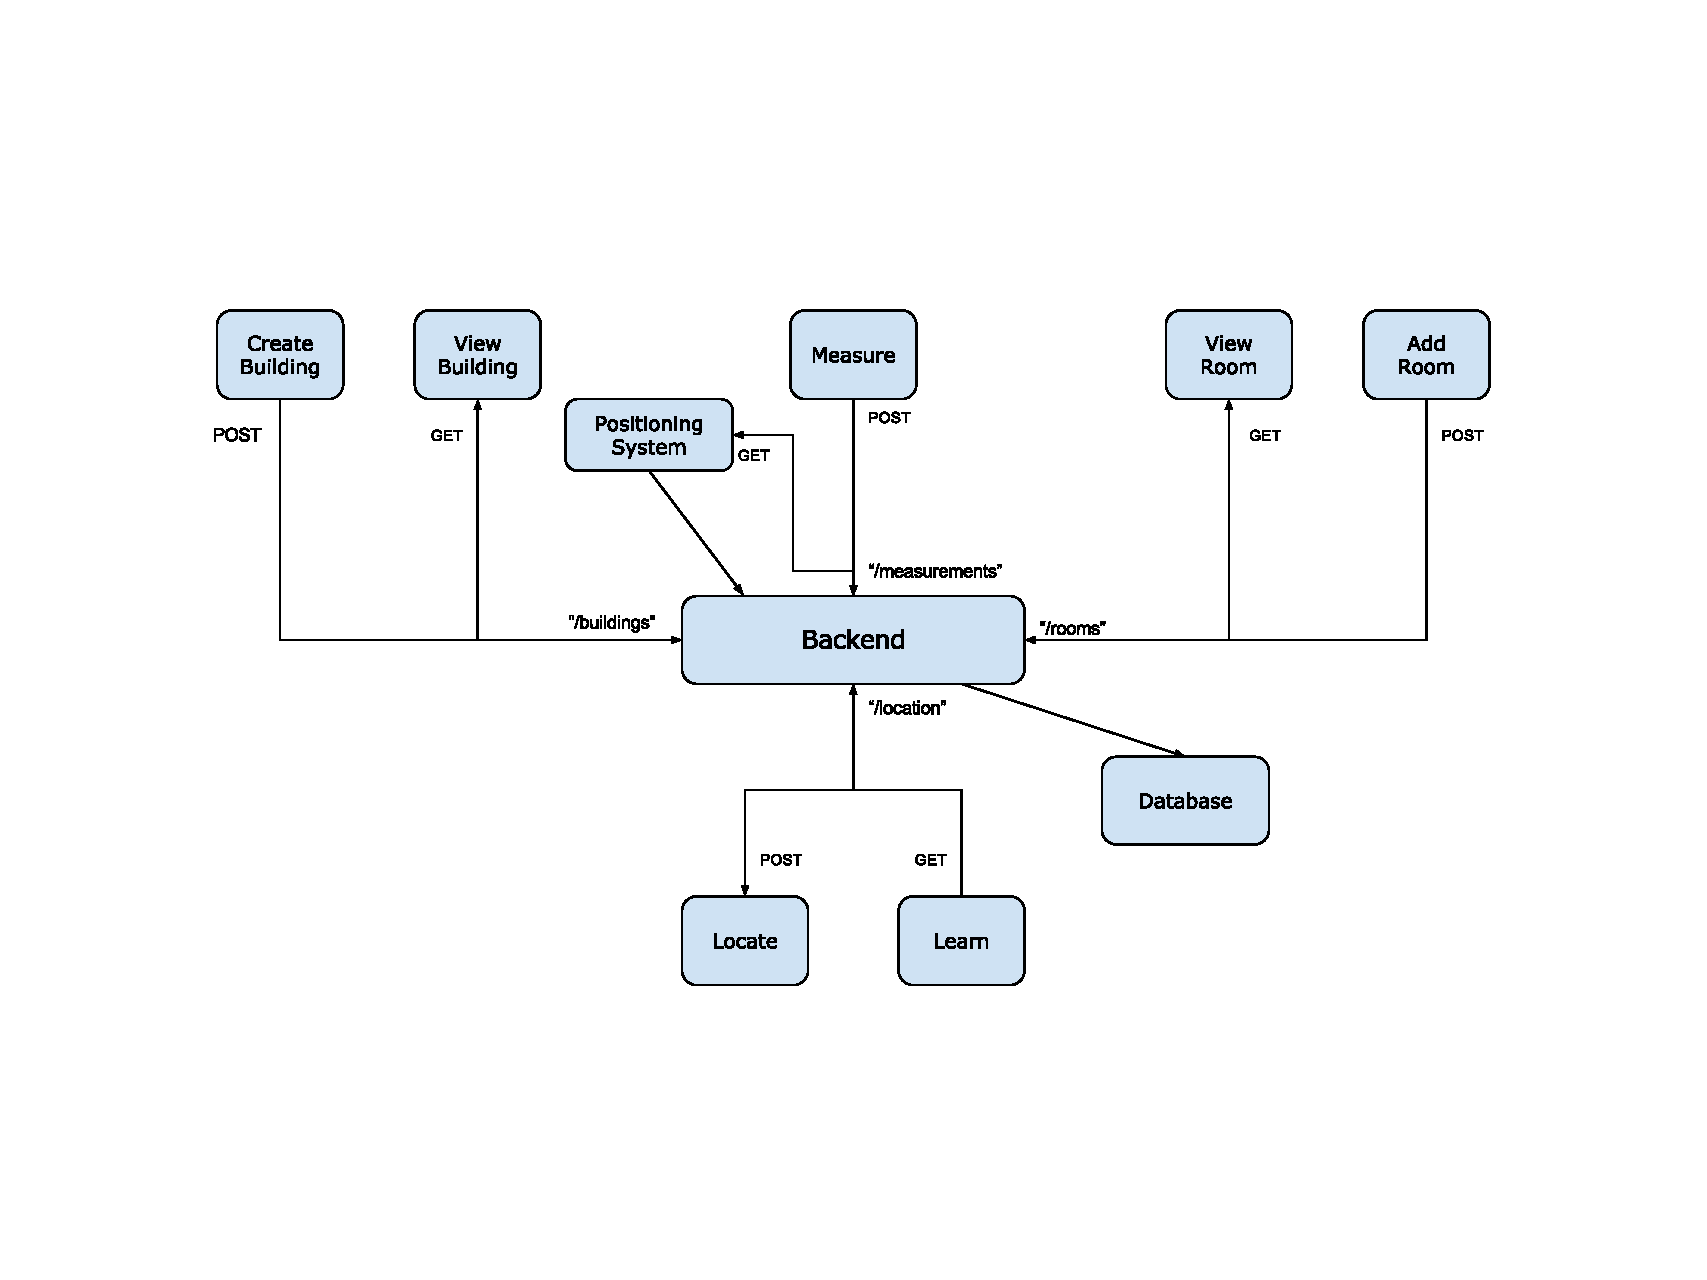
\includegraphics[width=\paperwidth]{DIAGRAMS/dataflow.pdf}}
\caption{Data Flow}
\end{figure}
The initial input is in the HOST android application. Here, the user inputs the details of a new building to be created. The data is then converted into JSON and sent to the Backend through a POST request to "/buildings". The backend parses the data and creates a new Building object, storing it in the database. The HOST then can select the building created and begin adding new room. For each new room, the details are entered and submitted. After submitting each room, the data, in JSON format, is sent to the Backend using a POST request to "/rooms/building\_id". The backend then created a new Room object, setting its building id to the specified id and storing it in the database. After the required rooms are added, the HOST must then take the RSS measurements for each room, in order for the classifier to be built. In the room activity, the HOST starts the measurements, and a list of all measurements taken at a point in time is then sent to the backend through a POST method to "measurements/room\_id", where the backend stores it in the database.
After enough measurements were taken for all the rooms, the host can then press the "learn" button from the building activity, which will send a GET request to "/locate/building\_id". On receipt of this request, the backend queries the database for all the measurements taken in the building and sends it through a TCP connection to the Positioning system, as a "learn" request. The positioning system processes the request and data, parsing it and storing the data locally. It will then initialise a classifier using the data stored, the system is then in standby again. \\
The next trigger is made by the VISITOR app, which, on start, will request a list of buildings from the backend using GET "/buildings/". The backend the queries and returns all the buildings stored. The user can then press on a building and see the list of rooms available. When the user starts a visit, a POST request is sent with the rooms and "want" levels that the user has specified to "/route/". The backend then sends a "route" request and forwards the data to the positioning system, which returns the suggested route. Finally, the app starts collecting RSS measurements. For every scan, the list of measurements is sent to the backend using a POST request to "/locate/building\_id". This triggers the backend to send a "classify" request to the positioning server, which returns a list of predicted locations. The backend the forwards the information back to the user.


\chapter{Implementation}
This chapter will go through the development process of the project. It will look into how the design was implemented, what changes have been made, some problems  faced along the way and how these problems were remediated.
\section{Development approach}
The project has taken a lean software development approach. The main goal was to achieve a prototype system, in order to test its feasibility. Therefore, some features were dropped or disregarded, as they were not crucial to the production of a testable system. The second principle of lean was also applied, analysing the value of the software based on its fitness to be used, rather than on the conformance to requirements. Therefore, focus was moved from documentation or planning towards coding, so that different ideas could be tried out and dropped if they proved infeasible, or if they did not increase the quality of the software. Another lean principle applied was giving the functionality of the system as a whole priority when developing each subsystem. Even though one of the objectives of the project is to create the subsystems as independent as possible, increasing reusability and flexibility to later changes, some compromises were made to ensure that the system as a whole was developed as soon as possible and was available for testing.

\noindent The following list shows, in order, the modules developed and the requirements targeted.

\begin{enumerate}
	\item Even though not a priority, the Visitor app was the first software created. The initial Android application was used to check whether the tools available through Google Indoor Maps API were usable for this project (V6, V7, V8).
	\item Data modelling classes were created in Java with some of the basic attributes and functionality (H1, H2, B1).
	\item Later on, more models were added and the classes became serializable to enable transmission of the objects.(H1, H2, B1).
	\item Data models for the positioning system were added (B2, H4).
	\item Work on backend started. A MySQL database was created and a Java class to connect and query the database was implemented (B1, B2).
	\item Tables were created in MySQL and Spatial Data Types were tested (B1, B2).
	\item NodeJS server, MongoDB and basic data models were created for experimentation (B1, B2, B3).
	\item The MySQL approach to the database was abandoned and data models were developed for MongoDB. The REST API was also developed to allow manipulation of the newly created database (B1, B2, B3).
	\item  Administration app was created (H1- H4).
	\item Java class for integrating with the API was implemented and added to the Administration app (H1-H4).
	\item Buildings Activity was implemented to show the list of all the buildings available (H1).
	\item Added building creation capability in the backend and in the Application's Database helper class (B1, H1).
	\item Building creation activity implemented in the Admin app (H1).
	\item Delete buildings and add rooms capabilities implemented in the Admin app (H1, H2).
	\item Positioning models implemented in the Backend and Database (B2).
	\item Wi-Fi scanning and posting measurements to server functionality implemented (H3, H4). 
	\item Positioning models changed for better inter-system compatibility.
	\item Basic Machine Learning functionality using Weka implemented and tested (PS2, PS4, PS5).
	\item Positioning server implemented after successful tests (PS1 - PS5).
	\item Added the Java Database helper class to the Visitor app (V1 - V8).
	\item Implemented Buildings, Room activities and started displaying current location of the device in Visitor App (V1, V3, V4, V7).	
	\item Implemented planner and JSON to PDDL parsing, returning a suggested route based on user specified requirements. (PS6, PS7)
	\item Input methods for visit requirements implemented in Visitor App (V3, V4, V5).
	\item Requesting and displaying suggested route generated by the Positioning Server (V6).
	\item Proximity sensing model added to the Backend.
	\item Proximity sensing implemented in the Visitor Application.
\end{enumerate}
The beginning of the implementation focused more on the Backend, in order to analyse the feasibility of different approaches. Once a basic version of the backend was implemented, the administration app was the next step in the implementation process. This allowed data to be inputted easier so that the rest of the system can be tested faster, when needed. The Backend and Database were tested using PostMan. Having Wi-Fi scanning capability early on helped understand the nature of the measurements, contributing to the design of the positioning system. The positioning system was implemented separately as a Java program and data was parsed and fed into the system manually for testing. Once the Positioning system proved feasible, data inputting became automated and the implementation moved its focus towards the Visitor app.

\section{Backend}
\subsection{Database and REST API}
Implementation of the backend was started by using a MySQL database. For easier administration MySQL Workbench software was used. A test database was created with two Tables. The first table, Building, contained five attributes: Name (VARCHAR), Width (INT), Length (INT), ID (INT) and Rectangle of type Geometry. The Geometry type is part of the Spatial Data Types offered in MySQL and it helps model and manage geometrical shapes ~\cite{MySql}.

Due to compatibility issues, the implementation of the backend moved to using a NodeJS server ~\cite{NodeJS} with a MongoDB database ~\cite{MongoDB}, which is the current implementation.
To ease implementation, Mongoose object modelling library was used when creating the Database models ~\cite{Mongoose}. The five models implemented and their corresponding schemas are shown below. 
\\
\textbf{Rectangle:}
This is a helper model to be used inside the other models, not to be instantiated on its own.
\begin{lstlisting}
{ lt:{x: Number, y: Number}, rt:{x: Number, y: Number}, 
lb:{x: Number, y: Number}, rb:{x: Number, y: Number} }	
\end{lstlisting}

\noindent
\textbf{Building:}
The building follows the model defined in the Design. 
\begin{lstlisting}
{ rectangle: Rectangle, name: {type: String, required: true},
width: {type: Number, required: true}, length:{type: Number, required: true} }
\end{lstlisting}

\noindent
\textbf{Room:}
Changes from the design were added here in order to implement the average visit time. The est\_time is given by calculating the average visit durations. For the average to be calculated, N\_avg stores the numbers of visits that the room has had.
\begin{lstlisting}
{ rectangle: Rectangle, name: {type: String, required: true},
width: {type: Number, required: true}, length:{type: Number, required: true},
floor: Number, est_time: {type: Number, default: 0}, N_avg: {type: Number,default:0},
building_id: {type: String, required: true} }
\end{lstlisting}

\noindent
\textbf{RP:}
The reference point model follows the definition in the Design. The rpid is stored as a string and is usually the MAC Address of the Wi-Fi access point.
\begin{lstlisting}
{ rpid: {type: String, required: true}, building_id: {type: String, required: true},
coordinate: {x: Number, y: Number} }
\end{lstlisting}

\noindent
\textbf{RPMeasurement:}
The rpv\_pair is an array that stores a list of RPID and the value measured. An array is needed because multiple access points can be detected in one scan. 
\begin{lstlisting}
{ rpv_pair: [{ RPID: String, value: Number }], 
room_id: {type: String, required: true} }
\end{lstlisting}

\noindent
\textbf{ExhibitRP:}
ExhibitRP stores the address of the bluetooth beacon associated to an exhibit, the name of the exhibit and the ID of the room in which it can be found.
\begin{lstlisting}
{ rpid: {type: String, required: true},
room_id: {type: String, required: true},
name: {type: String, required: true} }
\end{lstlisting}

The RESTful API was implemented using NodeJS and the ExpressJS Web Application framework ~\cite{ExpressJS}, for handling HTTP requests. The endpoints implemented followed the definition in Chapter 4.1.2 which will not be mentioned here to avoid repetition.

\subsection{Testing}
The backend was tested using the Postman Application. Requests were manually created and sent to the server, which ran locally. Further tests were made with the server running on a Virtual Machine hosted by DigitalOcean. No performance issues were noticed in either case.

Further tests were done during and after the development of the two Android Applications. The HTTP requests were made using the Java HttpURLConnection class.

\section{Positioning System}

\subsection{Server}
This class deals with receiving and sending data through a TCP connection to the Node Server. 
It contains an inner class, ClientThread, implementing Runnable, so that each request from the database is ran on a separate thread. The server waits for connections in a while(true) loop. When it receives a connection, it starts a new thread, instantiating a ClientThread object. A Buffered reader is used to read the data received from the node server. The data is in JSON format, therefore parsing must be done. The org.json library ~\cite{org.json} is used in order to parse the data. 
\begin{lstlisting} 
{"command":"learn","building_id":"id","learning_set":[]}
\end{lstlisting}
The first attribute looked at from the JSONObject received is "command", which can be  "learn", " classify" or "route". 
When a "learn" command is detected, the program will instantiate a classifier object for each classifier used. These objects are provided by Weka ~\cite{Weka} and include NaiveBayes, for the naive bayes classifier, or BayesNet, for the Bayes Network classifier. 
The classifiers are not instantiated by using "new", but they are returned by a static function call to Learner.learnFromJSON. This method takes as arguments the building id for which the learn command was called and a JSONArray containing the list of readings which will be used as the learning set. 
\begin{lstlisting} 
public static BayesNet learnFromJSON_BN(String building_id, JSONArray JSONData)
\end{lstlisting}
A global ArrayList storing Pairs ~\cite{tuple} of building id and classifier object is maintained. The list is used to minimise the number of times a classifier must be initialised. If the returned classifier from Learner.learnFromJSON has been previously initialised, the new object returned is introduced in the list using set, overwriting the previous object. If the classifier has not been previously initialised, it is added to the list using the add method. 
\begin{lstlisting}
//Check if a BayesNet classifier has been initialised.	
public int buildingClassifierBNInitialised(String building_id){
	for(Pair<String,BayesNet> p:classifiersBN){
		if(p.getLeft().equals(building_id))
        		return classifiersBN.indexOf(p);
        }
    return -1;
}    
\end{lstlisting}

\begin{lstlisting}
if(buildingClassifierBNInitialised(recJSON.getString("building_id")) > -1){
	classifiersBN.set(i,Pair.of(recJSON.getString("building_id"),bn));
} else {
	classifiersBN.add(Pair.of(recJSON.getString("building_id"),bn));
}
\end{lstlisting}

When a "classify" command is detected, the program will check whether any classifier has been initialised for the requested building. If none is found, it will check whether there is a learning set available for the specified building. If none is available, an error message will be returned. If a learning set is found, a classifier is then initialised through the same method as seen above for the "learn" command. Once the classifiers are available, they are passed, together with the unclassified data, to the static method Learner.classify. The method will return the classified room id, which in turn will be sent back to the Node server. Because the current system supports multiple types of classifiers, an array list must be declared for each type. The final value which is sent back to the Node server is formatted in such a way so as to allow the inclusion of all results. The format used is "CLASSIFIER:RESULT,CLASSIFIER:RESULT".
\begin{lstlisting}
String res ="BN:"+Learner.classify_BN(recJSON.getString("building_id"),
                  	recJSON.getJSONArray("learning_set"),classifiersBN.get(i).getRight());
res += ",NB:"+Learner.classify_NB(recJSON.getString("building_id"),
              	recJSON.getJSONArray("learning_set"),classifiersNB.get(j).getRight());
pw.write(res);
\end{lstlisting} 

When a "route" command is detected, the program will call the static method Planner.route(), passing the specifications, deadline and buildingID. The resulting route is received as a string and sent back to the Node server in the following format: 

\noindent "ACTION:ROOMS;ACTION:ROOMS;ACTION:ROOMS" where ACTION can be either "view" or "walk" and ROOMS is either the roomID to view, in case the action is "view", or the origin and destination roomIDs, separated by a comma, when the action is "walk".

\subsection{Learner}
As seen above, the Server class makes calls to static methods concerning the machine learning implementation. Those methods and other helper methods are implemented in the Learner class. In order for a classifier to be built and data to be classified, the Weka library requires data to be provided in an Attribute-Relation File Format (ARFF) file. Thus, the software must be able to parse the data from JSON and create an ARFF file to provide to the machine learning algorithm.

The static method learnFromJSON takes as arguments the building id for which the classifier will be built and the learning set as a JSONArray. Each element in the JSONArray is a Reading. A Reading contains two attributes, a String: "room\_id and a JSONArray:"rpv\_pair". The RPV Pair is a pair of Reference Point ID and Value. 
\begin{lstlisting}
//the learning set
"learning_set":[{"room_id":"room1408","rpv_pair":[The pairs go here]},{"room_id":"room237","rpv_pair":[Other pairs go here]}]

//Two rpv_pairs example
"rpv_pair":[{"RPID":"gr8:m8","value":-43},{"RPID":"n0:h8","value":-55}]
\end{lstlisting}

The program will create a list of all the RP IDs and Room IDs found in the data. Those lists will be stored in a file named "BuildingID\_RPs.data" for the RP IDs and in "BuildingID\_rooms.data" for the Rooms IDs. 

Once the files are created and saved, the program will start building the ARFF file. For each Reference Point, an attribute of NUMERIC Type is created: "@attribute RPID NUMERIC". Finally, an attribute of type NOMINAL for the class is added. "@attribute class \{RoomIDs\}. An attribute of nominal type can take one value from a finite set of possibilities. In our case, the possibilities are the RoomIDs. 

After defining the attributes needed, the data section must be inserted. The beginning of this section is marked by "@data". The data is inserted line by line. Each line is a list of comma separated measurement values, strictly in the order of the RPIDs defined in the attribute list, ending with the room id in which the reading was taken. After the ARFF file has been created, the classifier is initialised and returned to the caller.
\begin{lstlisting}
% ARFF file example

@relation room

@attribute gr8:m8 NUMERIC
@attribute n0:h8 NUMERIC
@attribute class {room1408, room237}

@data 
-43,-55,room1408
\end{lstlisting}

The static method classify has the same arguments as learnFromJSON, with the addition of the classifier object. 
\begin{lstlisting} 
public static String classify_BN(String building_id, JSONArray JSONdata, BayesNet bn)
\end{lstlisting}
The list of attributes is kept the same as in the previous method, with the difference being in the data. The data is only one line, because we are trying to classify based on one reading. Another difference is that, at the end of the line, a question mark is inserted instead of a room id. This file is saved with the name "buildingID\_temp.arff" and used to predict the RoomID, which is then returned to the caller. In order to facilitate concurrent calls to classify, temporary files must be created with different names, such as an index. After the method has finished, the program must delete the file so that the index gets freed.

The methods mentioned above must be able to apply different classifiers. Therefore, more than one method has been created for both learning and classifying, such as: learnFromJSON\_BN, learnFomJSON\_NB, classify\_NB and classify\_BN. 
\newpage

\subsection{Planner}
\begin{lstlisting}
public static String route(JSONArray jsonArray, int deadline, String building_id)
\end{lstlisting}
Visit route generation is implemented using the OPTIC planner ~\cite{OPTIC}. The planner takes as input two files: domain.pddl and problem.pddl. The domain file is predefined, whereas the problem file must be generated for each request. 
The domain defines two object types, exhibit and person: 
\begin{lstlisting}
(:types
    exhibit person - object
)
\end{lstlisting}
For each room in the request, an exhibit must be defined in the problem file. For the first room e0, for the second e1 and so on.
\begin{lstlisting}
(:objects
    visitor - person
    e0 e1 e2 - exhibit
)
\end{lstlisting}
The initial state is then defined by inserting what rooms the user wants to view, how long it takes for each room and how much the user wants to see a specific room. The deadline is finally inserted and goals are written. The file generated is named "buildingID\_temp.pddl". An example file can be found in Appendix B.
After the file is generated, the planner is executed with the two files as arguments. The planner running time could be very long, giving better and better solutions over time. As it was mentioned in the requirements, the route must be generated in less than 2 seconds, therefore the maximum time of execution for the planner was limited. The output of the planner is then parsed and returned as a String. 

\subsection{Testing}

The Machine Learning classifiers were initially tested by manually entering the data. A Java class was later created to automate a part of the data parsing. After the initial tests were completed, the current program was written, fully automating the parsing process. The Machine Learning algorithms were tested on different data sets throughout the development of the project. The final test results are shown and discussed in the Evaluation and Results chapter (6). 

The same principle applied to the testing of the Planning algorithm. Data for initial tests were manually entered. The current code was then written, automating the creation of the Problem PDDL file. The planner was first given 10, 5, 2 and 1 second to find a route. Running the planner for more than 1 second did not yield better results, therefore it was limited at a maximum execution time of 1 second, less than required in the specifications.

In both cases additional tests were done as part of Backend testing. Using Postman, requests were sent to check whether the requested data was correctly parsed and used and the outputs of the algorithms were correctly returned to the user.

\section{Administration App}
This is the main entry point to the system. The user can create buildings, add rooms and take measurements for the positioning system. In this part, we will look at the components of this app and their implementation. The classes included in the database, models and tools packages are used in both the administration and visitor app. Their implementations will be described in this section.

\subsection{Models and Tools Packages}
Following the design of the software, the data models are implemented in Java using the same attributes as the Backend models. One addition is the introduction of a Floor class, which can be later used for separating the building in floors. The current implementation does not use this model. The classes implement Serializable, to facilitate the transfer of data across activities. 

JUnit testing was performed to ensure that the models were correctly implemented. 
\subsection{Database}
The Database class offers a number of static methods that are used to connect to the Backend API. It handles HTTP connections, post and get requests and data parsing.

\noindent
The main HTTP functionality comes from two static methods:

\begin{lstlisting}
public static String getData(String... params)
\end{lstlisting}
This method builds a connection url using the parameters. The first parameter specifies the endpoint targeted (e.g.: buildings, rooms, etc.). The second parameter is optional and is used to specify the id, where needed. The request is sent to the server and the response is read using an InputStream. The method closes the connection and returns the data in JSON format, as a String.

\begin{lstlisting}
public static String postData(String... params)
\end{lstlisting}
In this method, the URL of the request is mostly built in the same way as in getData. The difference is that the first two parameters are obligatory. The first one is, like before, the request endpoint. The second parameter is the data to be sent. The third one is optional and specifies an id. 
In order for the data to be sent, we call
\begin{lstlisting}
connection.setDoOutput(true);
connection.setRequestProperty("Content-Type", "application/json");
\end{lstlisting}
The data is then converted to a byte array by calling getBytes() on the data String and written to the server using an OutputStream.
Because there is rarely any need for a call to these methods inside the Android activities, they are used mainly locally inside the class. The following methods are mainly used in both apps as the main way of interacting with the API.
\begin{lstlisting}
public static Building[] getBuildings();
public static Building getBuilding(String id);
public static boolean addBuilding(Building building);
public static Room[] getRooms(String building_id);
public static boolean addRoom(String building_id, Room room);
public static boolean postMeasurement(RPMeasurement measurement);
public static String classify(RPMeasurement measurement, String building_id);
public static String getRoute(String building_id, String rooms_exc, int deadline);
\end{lstlisting}
They parse received data from JSON instantiating Java Objects to be used inside the Activities or create JSON Objects from Java objects, in order for the data to be sent.

Tests were performed by sending mock data and monitoring the received data on the Backend side.
\subsection{MainActivity}
This is the entry activity to the app. It does not contain any important code, except a button which leads to the BuildingActivity. It was created as a way to access any activities that might branch out or that might not be accessible once the user is in BuildingActivity.

\subsection{BuildingsActivity}
In the current version of the app, this is the actual main activity, even though the app does not start from it.
The interface of this activity consists of a ListView and an Action Bar button with a "+" icon. 
The onResume activity has been overridden to fetch the buildings from the Database and add them to the ListView to be displayed and interacted with. The ListView has an OnItemClickListener attached, which reacts by starting the EditBuildingActivity. It is important to note that the building selected is passed to the next activity through intent.putExtra method. This is one of the uses of serializing the data models. When the user presses the action bar button, the AddBuildingActivity is started.

\subsection{EditBuildingActivity}
This activity consists of a form containing all the attributes found in the Building model and an action bar button for adding a new room. The form in this activity is not functional, because editing a building was not a high priority requirement. 
One use of the activity includes the user interaction with the list of rooms. The list is implemented in the same way as the list of buildings in BuildingsActivity. The difference is that onClick starts EditRoomActivity. Another difference is that, instead of passing the entire room object, the call passes only the RoomID.
The "Learn" button located above the ListView makes a call to Database.getData("learn", building\_id), sending a request to the positioning server to build a classifier for the building.
When the user presses the add button, AddRoomActivity is started.

\subsection{EditRoomActivity}
This activity was initially meant to serve as a way of editing the details of a building. After more considerations, the activity serves the purpose of collecting, displaying and sending to the server the Signal Strength measurements. 

In order for the measurements to be taken, the instance of WifiManager is accessed and a BroadcastReceiver is registered to handle the results of a WiFi scan.
\begin{lstlisting}
wifiManager = (WifiManager) getSystemService(Context.WIFI_SERVICE);
registerReceiver(broadcastReceiver, 
	new IntentFilter(WifiManager.SCAN_RESULTS_AVAILABLE_ACTION));
\end{lstlisting}
The Receiver takes the list of results and posts them to the Server. The control button, changes its text based on its current function. At the start of the activity it is displayed as "START". On click, it changes to "STOP" and so on. When the start function is called,  the boolean flag toMeasure is set to true and wifiManager.startScan() is called. After each scan has completed and the results posted, another call to wifiManager.startScan() is made in order to continue scanning. When the stop function is called, toMeasure is set to false and the next scan will not be explicitly called to start. Because the Android system issues scans without being explicitly asked, the activity will not post those measurements to the server, as they might have been taken in a different room than the one selected. 
\subsection{AddBuildingActivity}
This activity consists of a form and a submit button. The user completes the form with the details of the new building and, on submit, the format of the data is checked and the building is then sent to the Backend to be saved, with a call to Database.addBuilding(). After the data has been submitted, the activity terminates. 

\subsection{AddRoomActivity}
This is similar to the AddBuildingActivity. The difference is that, for faster testing, default values for the fields have been added. Another difference is that the data is posted to the server through a call to Database.addRoom(). 

Testing was performed by using all the functions of the application.
\section{Visitor App (Museum Guide)}
This is the Android application used by the visitors. It offers them the ability to view the buildings available and locate themselves once in one of the available buildings. As mentioned above, the Database and Models packages used in the Administration app are reused here with an identical implementation.

\subsection{MainActivity}
This is the application's entry point. It consists of a list of all the available buildings. The current building, if available, is shown at the top of the list and highlighted.  
When the user selects a building, the BuildingActivity is started, similar to the behaviour of BuildingsActivity in the Administration App.
\subsection{BuildingActivity}
This activity consists of a ListView of rooms, an EditText view, a TextView and a Button. Each item in the list contains a checkbox and a SeekBar. The user can select multiple rooms and use the SeekBar to choose the level of "excitement" (how much they would like to visit that specific room). When an item is selected, an estimated time of the visit is shown in a TextBox below. In order for the time estimation to be made available, the attribute was added to the models in both the Backend and Java. The average time for each room is calculated in the Backend. The EditText is used for the user to input the maximum time of the visit. Once the user is happy with their selection, the visit can be started by pressing the "GO" button. This button will then pass the required parameters and start GuideActivity.
\subsection{GuideActivity and MapsActivity}
As mentioned in the requirements, a visual aid must be given to the user concerning their current location and the suggested path. The current implementation of GuideActivty focuses on displaying this data as text, even though it is not the most user friendly approach. The models and system was built in such a way so that the buildings and rooms can be mapped on the global coordinates system. In order to enable visual information using Google Indoor Maps, the administration must enter the correct data of the buildings and rooms, such as Rectangle, in geographical coordinates. If this data is available, the MapsActivity should be started instead of GuideActivity. This will center the map to the requested building. The current location will be displayed as a marker on the center of the room.

Collecting signal strength measurements is implemented the same way as in the EditRoomActivity in the Admin App. The difference is that the user does not have the ability to stop the scans. After each scan has finished, the scan data is sent to the Backend to be classified, by calling Database.classify(). The result given is a list of multiple predictions. Here, a decision must be made on when to change the location and what location will be chosen if the predictions are different. Testing has been made using different approaches. To ensure precision, one approach is not changing the room at the exact moment a prediction shows a change. If the prediction shows that the room has been changed, the software can wait for 2 more predictions. If these predictions show the same room, then the position should be updated. The issue here is that the delay might be too long. The Android operating system does not allow an explicit call to start a scan, but rather hints the system to start scanning, when possible. Therefore, a delay can be quite long and the location can be changed multiple times while the app is still deciding whether the change is legitimate. This can lead to the system getting stuck indicating an outdated location. To fix this, updates can happen without making such checks. In the testing and evaluation section we will determine which approach is statistically the best, considering both precision and speed.

The application is also implementing Bluetooth capabilities in order to detect proximity. A Bluetooth beacon must be deployed and its Address associated to an exhibition. A threshold has been set in the application. If one of the registered beacons has a RSS bellow the threshold, the application will recognize proximity to the associated exhibition. 

In order for Bluetooth to work, the app firstly checks whether the phone is compatible or not and, if it is, then it checks whether Bluetooth is enabled. If Bluetooth is not enabled, a dialog is displayed asking the user to enable Bluetooth. A BroadcastReceiver is registered to handle the data of scans. Scans are started by calling startDiscovery().
\begin{lstlisting}
BluetoothAdapter bluetoothAdapter = BluetoothAdapter.getDefaultAdapter();
registerReceiver(btBroadcastReceiver, new IntentFilter(BluetoothDevice.ACTION_FOUND));
bluetoothAdapter.startDiscovery();
\end{lstlisting}

Testing was performed by using all the functions of the application.
\section{Implementation issues}
In order to determine the number and magnitude of the issues experienced during the development of an application, I usually look at how many keys and/or keyboards stopped working during the implementation phase. I am glad to say that, for this particular project, no keyboards were harmed. That is not to say that problems did no emerge along the way, nevertheless solutions were found quickly and pain-free. Below are some of the problems and solutions found, as far as I can remember, as most of the problems tend to arise in the middle of the night, when memory functions are not at their peak.

\subsection{Going back to previous Activity}
As seen before, when the users clicks on a building, the Building object selected is passed to the next activity, which uses the object as a global variable. The problem is that, when going back from the RoomActivity to the Building activity, by default Android instantiates another activity. Therefore, the global variable holding the Building passed from the list is going to be null and, when accessed, a NullPointerException is thrown. The solution was to set the launch mode of the BuildingAcitivty to "singleTask" in the Manifest file ~\cite{activity-element}. By doing so, the application can hold only one instance of that activity, which will always be on top of the activity stack, therefore saving all the local instances too.

\subsection{Bluetooth Scanning}
Scanning for Bluetooth devices is an expensive task so it must be used with care. I had not considered it to be an issue until I was forced to once I discovered that Android blocks further scans from being made if scans are requested too often. Therefore, scans must be initiated at predefined time intervals, and stopped once an exhibit is detected. Starting the scan was added into a TimerTask which is scheduled to run every 5 seconds.
\begin{lstlisting}
//timer task to start the scan every 5 seconds
TimerTask tt = new TimerTask() {
	@Override
    public void run() {
    		bluetoothAdapter.startDiscovery();
    }
};
new Timer().scheduleAtFixedRate(tt,0,5000);
        
//When an exhibit is detected, scanning is stopped.
if(device.getAddress().equals(currentExhibit) && rssi >= BLUETOOTH_THRESHOLD){
	bluetoothAdapter.cancelDiscovery();
}                      
        
\end{lstlisting}

\subsection{JavaScript callbacks} 
When the user chooses to press the Learn button in the Admin app, a request is sent to the Node server. The Node server must then query and prepare the data to be sent to the Positioning server. Because MonogoDB is a NoSql database, joins are not as straight forward. Therefore, in order to get all the RPMeasurements held for each Room inside a specific building, some form of nested loops are required. In this case, the first query returns all the rooms in one Building. For each room returned, a query is then made for all the RPMeasurements associated with that room. After writing the "straightforward" code, to my surprise, the data sent to the server was always empty. As this was my first time programming using JavaScript and NodeJS, I did not know that the queries are executed, by default, concurrently. This led to the subsequent queries to be executed before the previous queries finished. Because I was lacking experience, solving this problem took me quite some time, until I understood how to use callback functions, or at least I believe I understood them. The end solution looks like this:
\begin{lstlisting}
var rooms;
Room.find({'building_id': req.params.id}, function(err,data){
	rooms = data.map(function(data) {return data._id;});
    RPMeasurement.find({room_id: {$in: rooms}}, function(err,data){
    		request.learning_set = data;
        client.write(JSON.stringify(request));
        client.end();
    });
});
\end{lstlisting}

\subsection{Custom ListView}
Even though the Android SDK offers multiple options for implementing a ListView, a custom implementation was needed for the application. Each item in the list should contain a TextBox with the name of the room, a CheckBox to select the room for the visit and a SeekBar to allow the user to share how excited they are about visiting the room. 

To implement the specifications above, a custom XML layout was created containing the views. In addition to the layout, a custom ArrayAdapter was also implemented to handle user interactions. At the beginning the task seemed simple, until a problem arose when implementing the onClickListener for each item. The issue is that the action listener must be defined within the CustomAdapter class, instead of the Activity containing the ListView. As the estimated time is updated when the users selects or deselects a room, it was not possible to update the value any more, because the activity was not aware when selections occurred. 

To solve this problem, a public method was defined in BuildingActivity to update the Estimated Time.
\begin{lstlisting}
public void updateEstTime(){
        estTimeView.setText("Estimated time: " +(int) getEstTime());
    }
\end{lstlisting}
The method is called from within CustomAdapter when a selection occurs.
\begin{lstlisting}
checkBox.setOnClickListener(new View.OnClickListener() {
	@Override
    public void onClick(View v) {
        checked[(int) v.getTag()] = !checked[(int) v.getTag()];
        ((BuildingActivity) v.getContext()).updateEstTime();
    }
});
\end{lstlisting}
The estimated time is calculated in BuildingActivity:
\begin{lstlisting}
public double getEstTime(){
	double toReturn = 0;
    for(int i = 0;i<b.getRooms().length;++i){
    		if(((CustomAdapter) museumListView.getAdapter()).isChecked(i)){
        		toReturn+=b.getRooms()[i].getEst_time();
        }
    }
    return toReturn;
}
\end{lstlisting}
The method isChecked() called above is implemented in CustomAdapter:
\begin{lstlisting}
public boolean isChecked(int position) {
	return checked[position];
}
\end{lstlisting}
In short, CustomAdapter is implementing the listener and reacts when a selection is made by calling updateEstTime implemented in the Activity. The activity calculates the estimated time by checking which rooms are selected using isChecked() implemented in CustomAdapter.



\chapter{Results/Evaluation}
In this chapter we will review the performance of the resulting system and compare it with the requirements set in Chapter 3.
\section{IPS Performance Analysis}

The Java module implementing the Machine Learning algorithms uses only two types of classifiers, Naive Bayes and Bayes Network. Other classifiers were tested using the Weka GUI Explorer. 

Data was collected for two different buildings. The first set of data was taken in my personal flat. The surface area is approximately $55 m^2$ with all the rooms being close to each other. The rooms classified are: Kitchen, Bedroom, Living Room and Hallway. One assumption made was that, if the algorithm performance well in such a restricted environment, were the distance between rooms is quite limited, a better performance will be noticed in a larger space. The second set of data was taken at the Strand campus of King's College London. Because there was limited access to rooms and because of some people staring at a crazy looking guy walking around in circles talking to himself and lifting his phone in the air as if he was trying to film a concert or catch better signal, only a limited number of rooms were chosen for the test. After collecting the data, the classifiers were built and applied to the learning set. In order to get a more realistic result, the classifiers were also built with a part of the data, the rest being used as a test set.

In the flat tests, the fours rooms mention above were taken into account. 87 measurements were taken: 19 for room a, 24 for room b, 25 for room c and 19 for room d. Applying the built classifier to the learning set yielded the following results:

\noindent Naive Bayes:
\begin{lstlisting}
Time taken to build model: 0 seconds
=== Evaluation on training set ===
=== Summary ===
Correctly Classified Instances          87              100      %
Incorrectly Classified Instances         0                0      %
Total Number of Instances               87     
=== Confusion Matrix ===
  a  b  c  d   <-- classified as
 19  0  0  0 |  a
  0 24  0  0 |  b
  0  0 25  0 |  c
  0  0  0 19 |  d
\end{lstlisting}

\noindent Bayes Net:
\begin{lstlisting}
Time taken to build model: 0.01 seconds
=== Evaluation on training set ===
=== Summary ===
Correctly Classified Instances          86               98.8506 %
Incorrectly Classified Instances         1                1.1494 %
Total Number of Instances               87     
=== Confusion Matrix ===
  a  b  c  d   <-- classified as
 19  0  0  0 |  a
  0 24  0  0 |  b
  0  0 24  1 |  c
  0  0  0 19 |  d
\end{lstlisting}
The result show that the Naive Bayes algorithm classified all instances correctly were as Bayes Net had one error, when using the learning set as the test set.

A major difference in performance can be seen when separating the learning set from the training set. As it can be seen below, Bayes Networks perform much better in classifying the data, with only three errors.

\noindent Naive Bayes:
\begin{lstlisting}
Time taken to build model: 0 seconds
=== Evaluation on test set ===
=== Summary ===
Correctly Classified Instances          37               84.0909 %
Incorrectly Classified Instances         7               15.9091 %
Total Number of Instances               44     
=== Confusion Matrix ===
  a  b  c  d   <-- classified as
  9  0  0  0 |  a
  0 13  0  0 |  b
  0  0 13  2 |  c
  5  0  0  2 |  d
\end{lstlisting}

\noindent Naive Bayes:
\begin{lstlisting}
=== Evaluation on test set ===
=== Summary ===
Correctly Classified Instances          41               93.1818 %
Incorrectly Classified Instances         3                6.8182 %
Total Number of Instances               44     
=== Confusion Matrix ===
  a  b  c  d   <-- classified as
  8  1  0  0 |  a
  0 13  0  0 |  b
  0  0 13  2 |  c
  0  0  0  7 |  d


\end{lstlisting}

A worst case scenario test was taken, with only two instances for each room in the training set and 79 instances in the test set. The results show that, even with such a scarce learning set and large test set, Naive Bayes classified 60.7\% of instances correctly, and using Bayes Networks, 70.8\% of instances were correctly classified. It is important to mention that this worst case scenario is highly improbable.

In the strand campus case, three rooms were tested and 40 readings were taken in total: 8 readings for room a, 22 for room b and 10 for room c. Below are the results of applying the model on the learning set.

\noindent Naive Bayes:
\begin{lstlisting}
Time taken to build model: 0.02 seconds
=== Evaluation on training set ===
=== Summary ===
Correctly Classified Instances          40              100      %
Incorrectly Classified Instances         0                0      %
Total Number of Instances               40     
=== Confusion Matrix ===
  a  b  c   <-- classified as
  8  0  0 |  a
  0 22  0 |  b
  0  0 10 |  c
\end{lstlisting}

\noindent Bayes Net:
\begin{lstlisting}
Time taken to build model: 0.06 seconds
=== Evaluation on training set ===
=== Summary ===
Correctly Classified Instances          40              100      %
Incorrectly Classified Instances         0                0      %
Total Number of Instances               40     
=== Confusion Matrix ===
  a  b  c   <-- classified as
  8  0  0 |  a
  0 22  0 |  b
  0  0 10 |  c
\end{lstlisting}
As it can be seen, 100\% of instances were correctly classified using both classifiers, with a difference of 0.04 seconds in performance. 

In the second test, only 17 instances were used for learning and 23 instances were used for testing, the results being again 100\% for both types of classifiers. Because of such a high precision, the learning set was further reduced to 6 instances (2 for each room) and  the test set was increased to 34 instances, the result was again, 100\% for both types of classifiers.

The table below shows the results of other classifiers tested:

\begin{tabular}{ |p{3cm}|p{3cm}|p{3cm}|p{2cm}|p{2cm}| }
 \hline
 \multicolumn{5}{|c|}{Classifier Precision} \\
 \hline
 Classifier Type & Learning Set & Testing Set & Build time & Precision\\
 \hline
 Naive Bayes & 87 Instances & = Learning Set & 0s & 100\% \\
 Bayes Net   & 87 Instances & = Learning Set & 0.01s & 98.75\% \\
 KStar       & 87 Instances & = Learning Set & 0s & 100\% \\
 Decorate    & 87 Instances & = Learning Set & 0.7s & 100\% \\
 NB Trees    & 87 Instances & = Learning Set & 2.54 s & 100\% \\
 Naive Bayes & 42 Instances & 45 Instances & 0s & 86.66\% \\
 Bayes Net   & 42 Instances & 45 Instances & 0s & 93.33\% \\
 KStar       & 42 Instances & 45 Instances & 0s & 60\% \\
 Decorate    & 42 Instances & 45 Instances & 0.15s & 84.44\% \\
 NB Trees    & 42 Instances & 45 Instances & 0.01 s & 93.33\% \\
 Naive Bayes & 8 Instances & 78 Instances & 0s & 60.75\% \\
 Bayes Net   & 8 Instances & 78 Instances & 0s & 70.88\% \\
 KStar       & 8 Instances & 78 Instances & 0s & 40.50\% \\
 Decorate    & 8 Instances & 78 Instances & 0.01s & 51.89\% \\
 NB Trees    & 8 Instances & 78 Instances & 0.01s & 72.15\% \\
 \hline
\end{tabular}

\medskip \noindent Even though NBTrees show a higher precision when a scarce learning set is provided, the build time is quite high when a larger one is used. For 87 instances, a 2.54 second delay will affect the performance of the overall application. The delay would increase even higher if the a larger learning set would be given. Therefore, the best solution given the tests made is Bayes Net, and therefore this classifier will be used for the application.
It can also be seen that the precision of this system is higher than that shown be the system in Chapter 2. There, the best result was given by WKNN regression algorithm with 94.16\% which is comparable to the Bayes Net results when using only 42 instances. We can therefore assume that, given a larger learning set, such as the one provided in the system mentioned in Chapter 2, the results of using Bayes Net can be equal or even better.



\section{Section Heading}

\chapter{Professional and Ethical Issues}
The British Computing Society Code of Conduct was taken into account when developing the software. Other ethical issues were also considered and it was made sure that the resulting software does not infringe any rights of third parties, including and not limited to rights regarding privacy and intellectual property. 

The resulting software relies heavily on multiple libraries and tools developed by third parties, including but no limited to: the Weka collection of machine learning algorithms developed at The University of Waikato ~\cite{Weka}, OPTIC planner ~\cite{OPTIC} and the PDDL domain file which my supervisor helped me write, as I had limited knowledge in Planning. Other libraries were used throughout the software and can be seen in the code. 

Most of the data collected comes from user input. An exception is the collection and storage of Mac Addresses of the visible Wi-Fi access points and the signal strength measurements related. The duration of a visit for each room is uploaded and used to calculate the average visit time for each room. The average is stored but each visit's duration is not. All the data is anonymous and is not linked to any individual. 

As mentioned previously, no access control has yet been implemented and, therefore, the security of the system is very limited. All data held by the system is accessible. The next feature to be implemented will be security, and if anyone else should continue working on the system, I recommend they do the same.

The current implementation scans for all Wi-Fi access points, regardless of who owns them. This should not be an issue, as all Wi-Fi enabled devices do it, but storing the data might become an issue. If the system is used in a practical situation, the software must be changed to ensure that only the APs related to the building implementing the system are recorded.
\chapter{Conclusion and Future Work}

\section{Conclusion}
The difficulty of implementing a project without a team comes from the lack of diversity in skills that different team members would bring. This is also the best thing about working alone, as it requires people to learn new skills in order to reach their goals. 

During the development of this project, I had the chance to learn many things, from time and project management to new technologies and how to find and choose the right tools. I have learnt how to program using JavaScript and how to use NodeJS and other frameworks available to create a reliable and easy to develop backend. I have learnt about NoSql databases and how to model and query data efficiently using them. 
I have also improved my skills in Java and Android development by creating two mobile applications and a Java server. I have learnt about Machine Learning and its capabilities and limitations. I have learnt about Planning and PDDL, how to create a domain file and how to generate a problem file. The knowledge and skills gained through the individual project will help me throughout my career in Computer Science. It has been a difficult, but rewarding experience. 

The software developed in the project is far from complete. It was developed just as a first step towards a bigger project. It was used to prove the reliability of the idea and to provide a system which can be later extended and improved. It has been shown that, it is possible to determine, with high levels of precision, the indoor location of a Wi-Fi enabled device by using the already existing infrastructure. This means that no dedicated hardware is needed, greatly reducing the costs of implementing such a system in a real life scenario. It is also a great subject for future research into how precision can be further increased and, later on, accuracy. 
 
The next section will list some possible improvements that can be made to the existing software.

\section{Future Work}
\subsection{Security and Data collection}
The most important features that must be added to the next version are security related. Login methods must be implemented so that only the owners of a building can have access to the data stored. The idea behind this project doesn’t focus only on the usefulness for the visitors, but also for the hosts. It can be used by the management of museums to identify how people visit the museum, where they spend the most time and receive reviews at the end of the visits. It would help museums advertise their exhibits and improve their services. If such a system is to be developed, login methods must be implemented for visitors too. This would mean that issues concerning privacy will be raised. It is therefore important that such issues, which have not been addressed yet, will be addressed before the system becomes available to the public. 

\subsection{Graphics}
Another issue with the current implementation is the lack of a quality GUI. The interface is quite basic, just enough for the system to be used. It is important that a more practical and attractive interface is designed. This will help attract more users and improve the overall quality of the software. Graphics should also be implemented for displaying the indoor maps. It would allow hosts to easily create and manage the layout of their buildings and display to the visitors an interactive map, showing their locations, exhibits that can be viewed, more information about the exhibits that they are viewing and suggested paths that they can take for a better experience. 

\subsection{Optimisation}
Another weak point of the current implementation is its lack of optimisation. It is very likely that the current version would not be able to hold a large user base. The tools used in the implementation were not optimised for scalability. This means that, some modules, such as the planning and positioning system, must be modified to allow the handling of multiple simultaneous requests. Both android applications must also be optimised. Most importantly, the HTTP requests must be handled outside the UI thread. Caching should also be implemented to reduce the amount of data loaded from the internet. One approach can be to implement a broadcast system that checks whether data has been changed and updates the local cache when needed.

\subsection{Proximity interactions}
Even though the current implementation can identify when a visitor is viewing an exhibit, it does not offer any additional information. The app can be developed to show details about the exhibit being viewed. Cheaper methods for detecting viewers can also be added, such as QR Codes or NFC Tags. 



%%%%%%%%%%%%%%%%%%%%%%%%%%%%%%%%%
% References
%%%%%%%%%%%%%%%%%%%%%%%%%%%%%%%%%
\bibliographystyle{plain}
\bibliography{references}
\addcontentsline{toc}{section}{Bibliography}
\begin{thebibliography}{99}

\bibitem{Hofmann} B. Hofmann, H. Wellinhof, and H. Lichtenegger, ”GPS: Theory and Practice”, Springer-Verlag, Vienna, 1997.

\bibitem{Gu} Gu, Yanying, Anthony Lo, and Ignas Niemegeers. ”A survey of indoor positioning systems for wireless personal networks.” Communications Surveys Tutorials, IEEE 11.1 (2009):
13-32.

\bibitem{Golden} B.L. Golden, L. Levy, and R. Vohra. The orienteering problem. Naval Research Logistics, 34(3):307-318, 1987.

\bibitem{Flora} Di Flora, Cristiano, et al. ”Indoor and outdoor location based services for portable
wireless devices.” Distributed Computing Systems Workshops, 2005. 25th IEEE International
Conference on. IEEE, 2005

\bibitem{Hightower} J. Hightower and G. Borriello, ”Location sensing techniques”, Technical Report UW CSE 2001-07-30, Department of Computer Science and Engineering, University of Washington, 2001.

\bibitem{Depsey} M. Depsey, ”Indoor Positioning Systems in Healthcare”, Radianse Inc., White Paper, 2003, http://www.cimit.org/pubs/ips in healthcare.pdf.

\bibitem{Kaemarungsi} K. Kaemarungsi and P. Krishnamurthy, ”Properties of indoor received signal strength for WLAN location fingerprinting”, Proc. 1st Annual International Conference on Mobile and Ubiquitous Systems: Networking and Services (MobiQuitous ’04), Boston, Mass, USA, August 2004, pp. 14-23.

\bibitem{Small} J. Small, A. Smailagic, and D. P. Siewiorek, (2000, Dec.) Determining User Location For Context Aware Computing Through the Use of a Wireless LAN Infrastructure. [Online at] https://www.cs.cmu.edu/~aura/docdir/small00.pdf

\bibitem{Battiti} R. Battiti, M. Brunato, and A. Villani. (2002, Oct.) Statistical Learning Theory for Location Fingerprinting in Wireless LANs. Technical Report DIT-02-0086, Universit’a di Trento. [Online] Available: http://rtm.science.unitn.it/ ~battiti/archive/86.pdf

\bibitem{Murphy} https://datajobs.com/data-science-repo/Naive-Bayes-[Kevin-Murphy].pdf

\bibitem{Bishop} Bishop, C. (2006). Pattern recognition and machine learning. New York: Springer.

\bibitem{Want} R. Want, A. Hopper, V. Falcao, J. Gibbons, ”The Active Badge Location System”, ACM Trans. Information Systems, vol. 10, no. 1, January 1992, pp. 91-102.

\bibitem{ActiveBadge} Active Badge System, Website, 2008, http://www.cl.cam.ac.uk/research/dtg/attarchive/ab.html

\bibitem{AndroidCompat} http://static.googleusercontent.com/media/source.android.com/en//compatibility/android-cdd.pdf

\bibitem{Firefly1} Cybernet Interactive, Firefly Motion Capture System, 2008, http://www.cybernet.com/interactive/firefly/index.html 

\bibitem{Firefly2} ”Firefly Motion Tracking System User’s guide”, 1999, http://www.gesturecentral.com/firefly/FireflyUserGuide.pdf

\bibitem{Optotrak} http://www.ndigital.com/msci/products/optotrak-certus/

\bibitem{ActiveBat} Active Bat website, 2008, http://www.cl.cam.ac.uk/research/dtg/attarchive/

\bibitem{Priyantha1} N. Priyantha, A. Chakraborty, and H. Balakrishnan, ”The cricket location- support system”, Proc. ACM Conference on Mobile Computing and Networking, 2000. 

\bibitem{Priyantha2} N. B. Priyantha, ”The Cricket Indoor Location System”, PhD thesis, MIT, 2005.

\bibitem{Bahl} P. Bahl and V. Padmanabhan, ”RADAR: An in-building RF based user location and tracking system”, Proc. IEEE INFOCOM, vol. 2, March 2000, pp. 775-784.

\bibitem{Ekahau} Ekahau, 2008, http://www.ekahau.com/

\bibitem{King} T. King, S. Kopf, T. Haenselmann, C. Lubberger and W. Effelsberg, ”COMPASS: A Probabilistic Indoor Positioning System Based on 802.11 and Digital Compasses”, Proc. First ACM Intl Workshop on Wireless Network Testbeds, Experimental evaluation and CHara

\bibitem{Coles} Benton, J., Amanda Jane Coles, and Andrew Coles. "Temporal Planning with Preferences and Time-Dependent Continuous Costs." ICAPS. Vol. 77. 2012.

\bibitem{Bourke} http://paulbourke.net/geometry/circlesphere/


\bibitem{OPTIC} "http://www.inf.kcl.ac.uk/research/groups/PLANNING/index.php?option=com\_content\&view=article\&id=76\&Itemid=91"

\bibitem{Weka} http://www.cs.waikato.ac.nz/ml/weka/
\end{thebibliography}
%%%%%%%%%%%%%%%%%%%%%%%%%%%%%%%%%
% Appendices
%%%%%%%%%%%%%%%%%%%%%%%%%%%%%%%%%
\appendix
\include{Appendices/appendix}
\chapter{User Guide}
\section{Instructions}
To run the system please follow the steps below:
\begin{enumerate}
\item Start backend/nodeserver/server.js
\item Start backend/MLServer/MLServer.jar
\item Start IPS\_Admin app and create buildings+rooms.
\item Measure rooms using the IPS\_Admin. After the measurements are done, press the learn button in BuildingActivity
\item The MuseumGuide app can now be used to locate the device.
\end{enumerate}
\chapter{Source Code}
\section{Instructions}
Complete source code listings must be submitted as an appendix to the report. The project source codes are usually spread out over several files/units. You should try to help the reader to navigate through your source code by providing a ``table of contents'' (titles of these files/units and one line descriptions). The first page of the program listings folder must contain the following statement certifying the work as your own: ``I verify that I am the sole author of the programs contained in this folder, except where explicitly stated to the contrary''. Your (typed) signature and the date should follow this statement.

All work on programs must stop once the code is submitted to KEATS. You are required to keep safely several copies of this version of the program and you must use one of these copies in the project examination. Your examiners may ask to see the last-modified dates of your program files, and may ask you to demonstrate that the program files you use in the project examination are identical to the program files you have uploaded to KEATS. Any attempt to demonstrate code that is not included in your submitted source listings is an attempt to cheat; any such attempt will be reported to the KCL Misconduct Committee.

\textbf{You may find it easier to firstly generate a PDF of your source code using a text editor and then merge it to the end of your report. There are many free tools available that allow you to merge PDF files.}


\end{document}
